\section{Introduction}
\label{sec:introduction}

Robotic manipulation of dough and other elasto-plastic materials is challenging because each action alters both the observable geometry and the latent mechanical state of the material. This makes bimanual tool-based shaping particularly difficult: a controller must account for large deformations, complex contact interactions, rate-dependent behavior, and irreversible deformation that persists after unloading. Data-driven approaches can learn such behaviour from demonstrations or interaction data, but collecting broad physical datasets with robots is expensive. A calibrated simulator could instead generate controlled synthetic trajectories and support model-based action selection, provided that its predictions are tied to measurements of the real material.

\begin{figure*}[t]
    \centering
    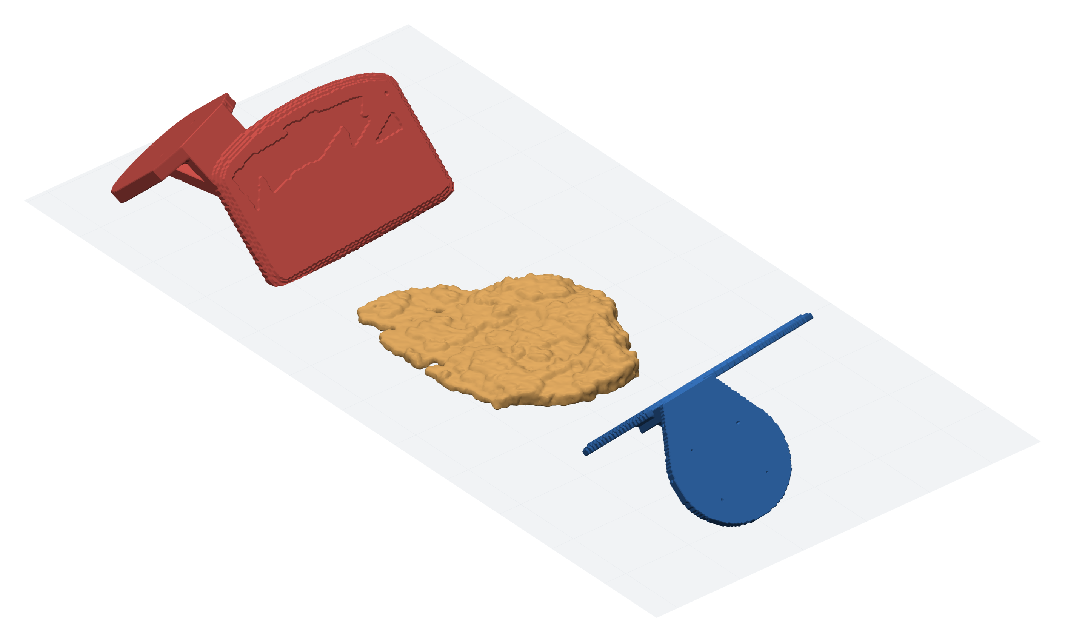
\includegraphics[width=0.6\textwidth]{figures/figure1_t0p5004.pdf}

    \captionsetup{width=0.6\textwidth}
    \caption{Simulation setup with both watertight spatula SDFs and reconstructed dough}
    \label{fig:simiulation}
\end{figure*}

In this work we introduce \textbf{TaichiDough}, a real-to-sim pipeline intended for future bimanual deformable object manipulation practices. A calibrated RGB-D camera records the dough while motion capture system (Mocap) provides the poses of both tools. The initial visible shape is reconstructed into a volumetric particle model, measured tool motion is replayed in a three-dimensional Material Point Method (MPM) simulator, and material parameters are adjusted to reduce disagreement between rendered and recorded depth observations. The same forward model supports a derivative-free Young's-modulus search and reverse-mode differentiation through complete trajectories.


% The central question is deliberately narrower than camera-based rheometry: what \emph{effective simulator parameters} can one calibrated view and known tool motion constrain? Absolute camera scale does not remove ambiguity among hidden volume, mass, contact, constitutive response, and numerical discretization. We therefore report parameter estimates only for the declared model and setup, and separate training loss from a frozen full-resolution evaluation. The robot execution and synthetic-data learning experiments are future work; the present study establishes and examines the identification pipeline that they require.



The contributions are:
\begin{itemize}
    \item a metric single-camera pipeline that combines floor-aware volumetric initialization;
    \item a differentiable MLS-MPM formulation for partial depth observations, including bounded optimizer coordinates for elastic, viscous, and principal-stretch parameters; and
\end{itemize}


\begin{figure*}[t]
    \centering
    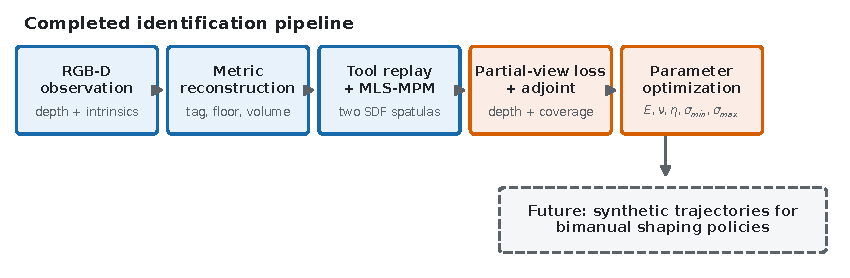
\includegraphics[width=0.98\textwidth]{figures/pipeline_overview.pdf}
    \caption{TaichiDough pipeline. A single calibrated RGB-D camera and recorded poses of two spatulas provide the initial geometry, observations, and boundary motion. A corrected MLS-MPM rollout is projected into the camera and compared with measured depth. Robot execution and synthetic-data learning are intended downstream uses rather than experiments reported here.}
    \label{fig:pipeline}
\end{figure*}

\section{Related Work}
\label{sec:related}

\textbf{Deformable object manipulation.}
Deformable object manipulation (DOM) spans linear, sheet-like, and
volumetric objects, including ropes, cloth, and dough
\cite{sanchez2018robotic,arriola2020modeling,yin2021modeling}.
To fit the simulator from the available single RGB-D view and measured
dual-tool trajectories, TaichiDough uses floor-aware volume
reconstruction and a depth-based objective, without requiring
multi-view appearance reconstruction. Physics-based approaches predict deformation
for planning \cite{jimenez2012survey}, whereas adaptive visual servoing
estimates motion--deformation relationships online
\cite{navarroalarcon2016automatic}. Learning-based methods train
policies or predictive models from demonstrations and interaction data
\cite{yin2021modeling}. G-DOOM combines learned latent graph dynamics
with model-predictive control for rope and cloth manipulation
\cite{ma2022learning}, showing that learned dynamics and model-based
control are compatible.

\textbf{Deformable simulation and differentiable physics.}
Simulation methods include mass--spring systems, finite-element
methods, position-based dynamics, smoothed particle hydrodynamics,
and the Material Point Method (MPM)
\cite{arriola2020modeling,yin2021modeling,jiang2016mpm}.
Mass--spring models are simple but depend on network parameterization;
finite-element methods discretize continuum models, while
position-based dynamics enforces geometric constraints
\cite{arriola2020modeling}. MPM accommodates large deformations
without a persistently deforming mesh while retaining constitutive
material models, motivating our choice for volumetric elasto-plastic
simulation \cite{jiang2016mpm}.
ChainQueen and DiffTaichi enable gradient-based optimization through
simulation \cite{hu2019chainqueen,hu2020difftaichi}, while PlasticineLab
applies differentiable physics to elasto-plastic manipulation
\cite{huang2021plasticinelab}. We use this capability in MLS-MPM to
fit material parameters to partial depth observations.

\textbf{Visual real-to-sim identification.}
Visual identification methods differ in sensing and geometric
assumptions. DiffCloud fits simulations to point clouds, whereas
Differentiable Depth uses a single depth camera and known reference
geometry \cite{sundaresan2022diffcloud,arnavaz2023diffdepth}.
PAC-NeRF jointly estimates geometry and physical parameters using
multi-view video and differentiable MPM \cite{li2023pacnerf};
PhysTwin reconstructs spring--mass digital twins from interaction
videos \cite{jiang2025phystwin}. DPSI identifies elasto-plastic material
and contact parameters from real interactions and incomplete point
clouds \cite{yang2025dpsi}, while EMPM combines multi-view RGB-D
reconstruction with online MPM parameter refinement
\cite{chen2026empm}. Within this literature, TaichiDough studies a
calibrated single-view setting with floor-aware volume reconstruction,
measured dual-tool trajectories, and depth-based fitting.

\textbf{Robotic shaping and dough mechanics.}
RoboCraft and RoboCook learn predictive dynamics for goal-directed
shaping and manipulation with diverse tools
\cite{shi2022robocraft,shi2023robocook}, while DoughNet predicts
geometric and topological changes \cite{bauer2024doughnet}.
Complementary food-engineering studies estimate dough rheology through
controlled mechanical measurements; Fabbri and Cevoli combine
finite-element model inversion with extrusion measurements
\cite{fabbri2015dough}. Dough response depends on formulation,
loading, preparation, and adhesion
\cite{yazar2023doughreview,ghorbel2014adhesion}.
Accordingly, our fitted parameters characterize the selected
constitutive and contact model over the recorded manipulation,
rather than providing a complete rheological characterization.